\documentclass{article}\usepackage[]{graphicx}\usepackage[table]{xcolor}
% maxwidth is the original width if it is less than linewidth
% otherwise use linewidth (to make sure the graphics do not exceed the margin)
\makeatletter
\def\maxwidth{ %
  \ifdim\Gin@nat@width>\linewidth
    \linewidth
  \else
    \Gin@nat@width
  \fi
}
\makeatother

\definecolor{fgcolor}{rgb}{0.345, 0.345, 0.345}
\newcommand{\hlnum}[1]{\textcolor[rgb]{0.686,0.059,0.569}{#1}}%
\newcommand{\hlsng}[1]{\textcolor[rgb]{0.192,0.494,0.8}{#1}}%
\newcommand{\hlcom}[1]{\textcolor[rgb]{0.678,0.584,0.686}{\textit{#1}}}%
\newcommand{\hlopt}[1]{\textcolor[rgb]{0,0,0}{#1}}%
\newcommand{\hldef}[1]{\textcolor[rgb]{0.345,0.345,0.345}{#1}}%
\newcommand{\hlkwa}[1]{\textcolor[rgb]{0.161,0.373,0.58}{\textbf{#1}}}%
\newcommand{\hlkwb}[1]{\textcolor[rgb]{0.69,0.353,0.396}{#1}}%
\newcommand{\hlkwc}[1]{\textcolor[rgb]{0.333,0.667,0.333}{#1}}%
\newcommand{\hlkwd}[1]{\textcolor[rgb]{0.737,0.353,0.396}{\textbf{#1}}}%
\let\hlipl\hlkwb

\usepackage{framed}
\makeatletter
\newenvironment{kframe}{%
 \def\at@end@of@kframe{}%
 \ifinner\ifhmode%
  \def\at@end@of@kframe{\end{minipage}}%
  \begin{minipage}{\columnwidth}%
 \fi\fi%
 \def\FrameCommand##1{\hskip\@totalleftmargin \hskip-\fboxsep
 \colorbox{shadecolor}{##1}\hskip-\fboxsep
     % There is no \\@totalrightmargin, so:
     \hskip-\linewidth \hskip-\@totalleftmargin \hskip\columnwidth}%
 \MakeFramed {\advance\hsize-\width
   \@totalleftmargin\z@ \linewidth\hsize
   \@setminipage}}%
 {\par\unskip\endMakeFramed%
 \at@end@of@kframe}
\makeatother

\definecolor{shadecolor}{rgb}{.97, .97, .97}
\definecolor{messagecolor}{rgb}{0, 0, 0}
\definecolor{warningcolor}{rgb}{1, 0, 1}
\definecolor{errorcolor}{rgb}{1, 0, 0}
\newenvironment{knitrout}{}{} % an empty environment to be redefined in TeX

\usepackage{alltt}

\usepackage[utf8]{inputenc}
\usepackage{float}
\usepackage{graphicx}
\usepackage{booktabs}
\usepackage[table]{xcolor}
\IfFileExists{upquote.sty}{\usepackage{upquote}}{}
\begin{document}
Se realizara el analisis de las encuestas de todas la encuestas realizadas en el trabajo de campo.\\


\begin{tabular}{lcl}
\toprule
\cellcolor[HTML]{87A96B}{\textcolor{black}{\textbf{Rango}}} & \cellcolor[HTML]{87A96B}{\textcolor{black}{\textbf{Conteo}}} & \cellcolor[HTML]{87A96B}{\textcolor{black}{\textbf{Porcentaje}}}\\
\midrule
(23.9,33.3] & 28 & 6.35\\
(33.3,42.6] & 54 & 12.24\\
(42.6,51.9] & 87 & 19.73\\
(51.9,61.1] & 127 & 28.80\\
(61.1,70.4] & 97 & 22.00\\
\addlinespace
(70.4,79.7] & 35 & 7.94\\
(79.7,89.1] & 13 & 2.95\\
\bottomrule
\end{tabular}

Aca ira la interpretacion de la tabla
\begin{knitrout}
\definecolor{shadecolor}{rgb}{0.969, 0.969, 0.969}\color{fgcolor}
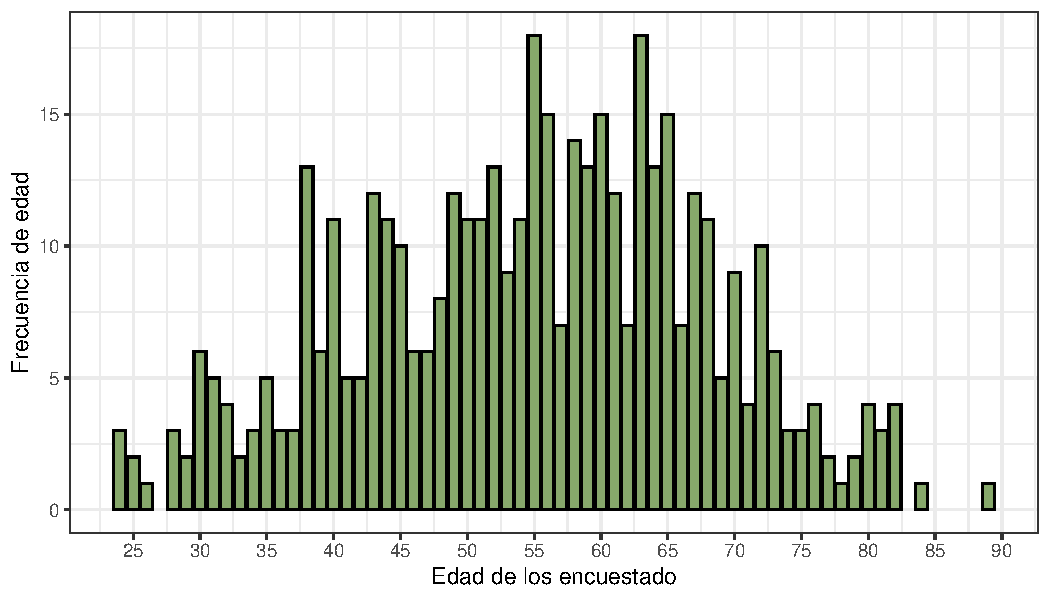
\includegraphics[width=\maxwidth]{figure/fig_uno-1} 
\end{knitrout}
mas interpretacion de la grafica

\begin{figure}[H]
  \centering
  \caption{Aplicando encuesta}
  \includegraphics[scale=0.5]{C:/Users/PERCY/Desktop/img000001.png}
  \caption*{Fuente: trabajo de campo}
\end{figure}

\end{document}
